\begin{center}
  \begin{figure}[H]
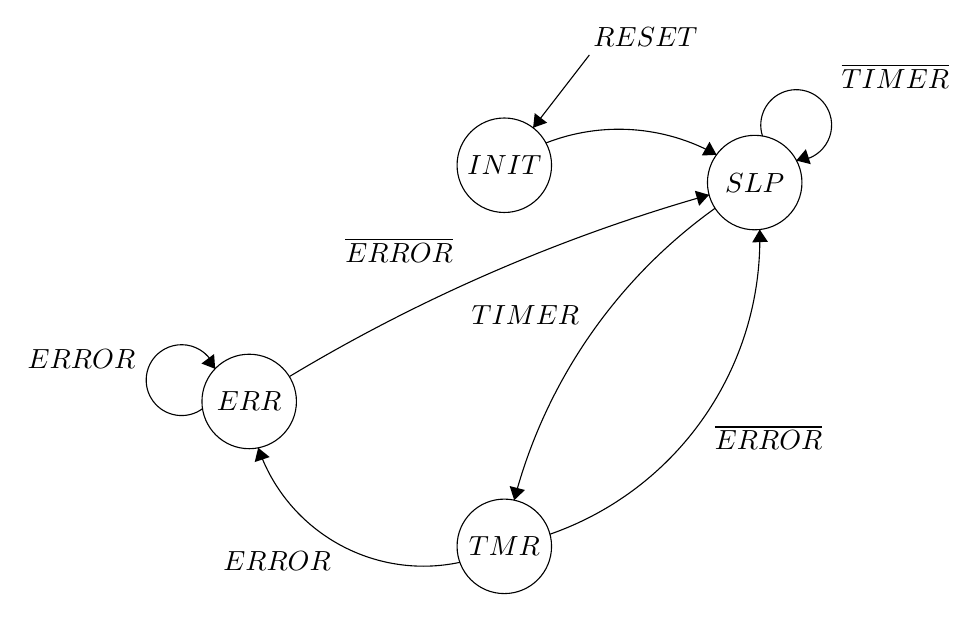
\begin{tikzpicture}[scale=0.2]
\tikzstyle{every node}+=[inner sep=0pt]
\draw [black] (31.1,-9.2) circle (3);
\draw (31.1,-9.2) node {$INIT$};
\draw [black] (47,-10.3) circle (3);
\draw (47,-10.3) node {$SLP$};
\draw [black] (31.1,-33.4) circle (3);
\draw (31.1,-33.4) node {$TMR$};
\draw [black] (14.9,-24.2) circle (3);
\draw (14.9,-24.2) node {$ERR$};
\draw [black] (36.5,-2.2) -- (32.93,-6.82);
\draw (40.06,-1.7) node [above] {$RESET$};
\fill [black] (32.93,-6.82) -- (33.82,-6.5) -- (33.03,-5.89);
\draw [black] (47.497,-7.353) arc (198.16235:-89.83765:2.25);
\draw (55.93,-4.33) node [above] {$\overline{TIMER}$};
\fill [black] (49.64,-8.9) -- (50.56,-9.13) -- (50.25,-8.18);
\draw [black] (31.726,-30.467) arc (165.34976:125.57006:33.07);
\fill [black] (31.73,-30.47) -- (32.41,-29.82) -- (31.44,-29.57);
\draw (35.88,-18.73) node [left] {$TIMER$};
\draw [black] (28.286,-34.414) arc (-77.93441:-161.25018:11.087);
\fill [black] (15.47,-27.14) -- (15.25,-28.05) -- (16.2,-27.73);
\draw (16.67,-33.72) node [below] {$ERROR$};
\draw [black] (17.45,-22.62) arc (121.01029:105.81704:109.852);
\fill [black] (44.1,-11.08) -- (43.2,-10.82) -- (43.47,-11.78);
\draw (24.42,-15.39) node [above] {$\overline{ERROR}$};
\draw [black] (33.739,-7.787) arc (111.3961:60.68879:12.691);
\fill [black] (44.58,-8.54) -- (44.13,-7.71) -- (43.64,-8.58);
\draw [black] (47.316,-13.28) arc (1.72743:-70.80761:19.856);
\fill [black] (47.32,-13.28) -- (46.84,-14.1) -- (47.84,-14.06);
\draw (44.43,-26.49) node [right] {$\overline{ERROR}$};
\draw [black] (11.946,-24.654) arc (306.47443:18.47443:2.25);
\draw (7.7,-21.52) node [left] {$ERROR$};
\fill [black] (12.74,-22.13) -- (12.67,-21.19) -- (11.87,-21.79);
\end{tikzpicture}
\caption{Functional State Diagram: Sub Unit}
\label{fig:fsd-sub}
\end{figure}
\begin{table}[h!]
  \begin{tabular}{c|c}
    STATE&OUTPUTS\\
    \hline
    &\\
    INIT&$\overline{REPORT}\hbox{  }\hbox{  }\hbox{  }\overline{TIMER}\hbox{  }\hbox{  }\hbox{  }POWER\hbox{ }\hbox{  }\hbox{  }\overline{ERROR}\hbox{  }\hbox{  }\hbox{  }\overline{RED}$\\
    SLP&$\overline{REPORT}\hbox{  }\hbox{  }\hbox{  }\overline{TIMER}\hbox{  }\hbox{  }\hbox{  }POWER\hbox{ }\hbox{  }\hbox{  }\overline{ERROR}\hbox{  }\hbox{  }\hbox{  }\overline{RED}$\\
    TMR&$\overline{REPORT}\hbox{  }\hbox{  }\hbox{  }TIMER\hbox{  }\hbox{  }\hbox{  }POWER\hbox{ }\hbox{  }\hbox{  }\overline{ERROR}\hbox{  }\hbox{  }\hbox{  }\overline{RED}$\\
    ERR&$REPORT\hbox{  }\hbox{  }\hbox{  }TIMER\hbox{  }\hbox{  }\hbox{  }POWER\hbox{ }\hbox{  }\hbox{  }ERROR\hbox{  }\hbox{  }\hbox{  }RED$\\
  \end{tabular}
  \caption{Functional State Diagram Sub Unit: State and Outputs}
  \label{fig:fsd-sub-state-outputs}
\end{table}
\begin{table}[h!]
  \begin{tabular}{|c|}
    \hline
    Output List\\
    \hline
    ERROR = Send temperature related errors or warnings via Bluetooth module\\
    TIMER = RTC ISR has been called\\
    RED = Red LED is lit up\\
    \hline
  \end{tabular}
  \caption{Functional State Diagram Main Unit: Output List}
  \label{fig:fsd-sub-output-list}
\end{table}
\end{center}
